% Replicates: Adler et al., arXiv:2510.16060v2 (27 May 2026). All numbers below come from results/*.csv via
% scripts/make_tables.py (tables/*.tex, tables/numbers.tex) unless quoted from the paper with a table reference.
\newcommand{\maxTSFMpceCrime}{0.035}
\newcommand{\minTSFMpceCrime}{0.023}
\newcommand{\nTSFMCrime}{4}
\newcommand{\pceCsCrime}{0.024}
\newcommand{\cceCsCrime}{-0.006}
\newcommand{\maseCsCrime}{0.802}
\newcommand{\pceCbCrime}{0.035}
\newcommand{\cceCbCrime}{-0.011}
\newcommand{\maseCbCrime}{0.805}
\newcommand{\pceTfmCrime}{0.027}
\newcommand{\cceTfmCrime}{-0.016}
\newcommand{\maseTfmCrime}{0.783}
\newcommand{\pceTrxCrime}{0.023}
\newcommand{\cceTrxCrime}{-0.049}
\newcommand{\maseTrxCrime}{0.788}
\newcommand{\pceArimaCrime}{0.065}
\newcommand{\cceArimaCrime}{-0.140}
\newcommand{\maseArimaCrime}{1.029}
\newcommand{\pceArimaTCrime}{0.024}
\newcommand{\cceArimaTCrime}{-0.041}
\newcommand{\maseArimaTCrime}{0.942}
\newcommand{\pceArimaGCrime}{0.065}
\newcommand{\cceArimaGCrime}{-0.140}
\newcommand{\maseArimaGCrime}{1.029}
\newcommand{\pceNbeatsCrime}{0.199}
\newcommand{\cceNbeatsCrime}{0.443}
\newcommand{\maseNbeatsCrime}{0.976}
\newcommand{\pceNbeatsHCrime}{0.058}
\newcommand{\cceNbeatsHCrime}{0.123}
\newcommand{\maseNbeatsHCrime}{0.859}
\newcommand{\pceNbeatsFoneCrime}{0.200}
\newcommand{\cceNbeatsFoneCrime}{0.446}
\newcommand{\maseNbeatsFoneCrime}{0.975}
\newcommand{\pceNbeatsFHoneCrime}{0.034}
\newcommand{\cceNbeatsFHoneCrime}{0.011}
\newcommand{\maseNbeatsFHoneCrime}{0.830}
\newcommand{\pcewinTSFMminCrime}{0.109}
\newcommand{\nwinCrime}{4{,}030}
\newcommand{\nserCrime}{5}
\newcommand{\maxTSFMpceGlucose}{0.033}
\newcommand{\minTSFMpceGlucose}{0.028}
\newcommand{\nTSFMGlucose}{4}
\newcommand{\pceCsGlucose}{0.030}
\newcommand{\cceCsGlucose}{-0.028}
\newcommand{\maseCsGlucose}{7.263}
\newcommand{\pceCbGlucose}{0.033}
\newcommand{\cceCbGlucose}{-0.016}
\newcommand{\maseCbGlucose}{7.292}
\newcommand{\pceTfmGlucose}{0.028}
\newcommand{\cceTfmGlucose}{-0.029}
\newcommand{\maseTfmGlucose}{6.567}
\newcommand{\pceTrxGlucose}{0.031}
\newcommand{\cceTrxGlucose}{-0.028}
\newcommand{\maseTrxGlucose}{6.500}
\newcommand{\pceArimaGlucose}{0.055}
\newcommand{\cceArimaGlucose}{-0.022}
\newcommand{\maseArimaGlucose}{1.8e5}
\newcommand{\pceArimaTGlucose}{0.067}
\newcommand{\cceArimaTGlucose}{-0.102}
\newcommand{\maseArimaTGlucose}{8.476}
\newcommand{\pceArimaGGlucose}{0.055}
\newcommand{\cceArimaGGlucose}{-0.019}
\newcommand{\maseArimaGGlucose}{8.472}
\newcommand{\pceNbeatsGlucose}{0.212}
\newcommand{\cceNbeatsGlucose}{0.460}
\newcommand{\maseNbeatsGlucose}{8.584}
\newcommand{\pceNbeatsHGlucose}{0.054}
\newcommand{\cceNbeatsHGlucose}{0.099}
\newcommand{\maseNbeatsHGlucose}{7.862}
\newcommand{\pceNbeatsFoneGlucose}{0.212}
\newcommand{\cceNbeatsFoneGlucose}{0.460}
\newcommand{\maseNbeatsFoneGlucose}{8.673}
\newcommand{\pceNbeatsFHoneGlucose}{0.051}
\newcommand{\cceNbeatsFHoneGlucose}{0.096}
\newcommand{\maseNbeatsFHoneGlucose}{7.814}
\newcommand{\pcewinTSFMminGlucose}{0.197}
\newcommand{\nwinGlucose}{13{,}040}
\newcommand{\nserGlucose}{16}
\newcommand{\maxTSFMpceHR}{0.055}
\newcommand{\minTSFMpceHR}{0.036}
\newcommand{\nTSFMHR}{4}
\newcommand{\pceCsHR}{0.053}
\newcommand{\cceCsHR}{-0.060}
\newcommand{\maseCsHR}{1.549}
\newcommand{\pceCbHR}{0.055}
\newcommand{\cceCbHR}{-0.070}
\newcommand{\maseCbHR}{1.549}
\newcommand{\pceTfmHR}{0.036}
\newcommand{\cceTfmHR}{-0.000}
\newcommand{\maseTfmHR}{1.465}
\newcommand{\pceTrxHR}{0.043}
\newcommand{\cceTrxHR}{-0.050}
\newcommand{\maseTrxHR}{1.461}
\newcommand{\pceArimaHR}{0.066}
\newcommand{\cceArimaHR}{-0.131}
\newcommand{\maseArimaHR}{1.842}
\newcommand{\pceArimaTHR}{0.055}
\newcommand{\cceArimaTHR}{-0.100}
\newcommand{\maseArimaTHR}{1.591}
\newcommand{\pceArimaGHR}{0.066}
\newcommand{\cceArimaGHR}{-0.131}
\newcommand{\maseArimaGHR}{1.842}
\newcommand{\pceNbeatsHR}{0.208}
\newcommand{\cceNbeatsHR}{0.432}
\newcommand{\maseNbeatsHR}{1.640}
\newcommand{\pceNbeatsHHR}{0.059}
\newcommand{\cceNbeatsHHR}{0.016}
\newcommand{\maseNbeatsHHR}{1.538}
\newcommand{\pceNbeatsFoneHR}{0.206}
\newcommand{\cceNbeatsFoneHR}{0.429}
\newcommand{\maseNbeatsFoneHR}{1.640}
\newcommand{\pceNbeatsFHoneHR}{0.059}
\newcommand{\cceNbeatsFHoneHR}{0.016}
\newcommand{\maseNbeatsFHoneHR}{1.538}
\newcommand{\pcewinTSFMminHR}{0.132}
\newcommand{\nwinHR}{1{,}794}
\newcommand{\nserHR}{6}
\newcommand{\maxTSFMpceRev}{0.014}
\newcommand{\minTSFMpceRev}{0.010}
\newcommand{\nTSFMRev}{4}
\newcommand{\pceCsRev}{0.011}
\newcommand{\cceCsRev}{-0.007}
\newcommand{\maseCsRev}{0.797}
\newcommand{\pceCbRev}{0.014}
\newcommand{\cceCbRev}{-0.012}
\newcommand{\maseCbRev}{0.797}
\newcommand{\pceTfmRev}{0.011}
\newcommand{\cceTfmRev}{0.007}
\newcommand{\maseTfmRev}{0.770}
\newcommand{\pceTrxRev}{0.010}
\newcommand{\cceTrxRev}{-0.010}
\newcommand{\maseTrxRev}{0.786}
\newcommand{\pceArimaRev}{0.058}
\newcommand{\cceArimaRev}{-0.108}
\newcommand{\maseArimaRev}{41.287}
\newcommand{\pceArimaTRev}{0.057}
\newcommand{\cceArimaTRev}{-0.118}
\newcommand{\maseArimaTRev}{7.8e4}
\newcommand{\pceArimaGRev}{n/a}
\newcommand{\cceArimaGRev}{n/a}
\newcommand{\maseArimaGRev}{n/a}
\newcommand{\pceNbeatsRev}{n/a}
\newcommand{\cceNbeatsRev}{n/a}
\newcommand{\maseNbeatsRev}{n/a}
\newcommand{\pceNbeatsHRev}{n/a}
\newcommand{\cceNbeatsHRev}{n/a}
\newcommand{\maseNbeatsHRev}{n/a}
\newcommand{\pceNbeatsFoneRev}{0.066}
\newcommand{\cceNbeatsFoneRev}{0.141}
\newcommand{\maseNbeatsFoneRev}{1.028}
\newcommand{\pceNbeatsFHoneRev}{0.046}
\newcommand{\cceNbeatsFHoneRev}{0.075}
\newcommand{\maseNbeatsFHoneRev}{1.170}
\newcommand{\pcewinTSFMminRev}{0.122}
\newcommand{\nwinRev}{358{,}610}
\newcommand{\nserRev}{235}
\newcommand{\maxTSFMpceMfive}{0.053}
\newcommand{\minTSFMpceMfive}{0.040}
\newcommand{\nTSFMMfive}{4}
\newcommand{\pceCsMfive}{0.046}
\newcommand{\cceCsMfive}{0.034}
\newcommand{\maseCsMfive}{0.775}
\newcommand{\pceCbMfive}{0.040}
\newcommand{\cceCbMfive}{0.010}
\newcommand{\maseCbMfive}{0.763}
\newcommand{\pceTfmMfive}{0.053}
\newcommand{\cceTfmMfive}{0.008}
\newcommand{\maseTfmMfive}{0.722}
\newcommand{\pceTrxMfive}{0.042}
\newcommand{\cceTrxMfive}{-0.020}
\newcommand{\maseTrxMfive}{0.740}
\newcommand{\pceArimaMfive}{0.049}
\newcommand{\cceArimaMfive}{-0.086}
\newcommand{\maseArimaMfive}{1.075}
\newcommand{\pceArimaTMfive}{0.040}
\newcommand{\cceArimaTMfive}{-0.020}
\newcommand{\maseArimaTMfive}{0.897}
\newcommand{\pceArimaGMfive}{n/a}
\newcommand{\cceArimaGMfive}{n/a}
\newcommand{\maseArimaGMfive}{n/a}
\newcommand{\pceNbeatsMfive}{n/a}
\newcommand{\cceNbeatsMfive}{n/a}
\newcommand{\maseNbeatsMfive}{n/a}
\newcommand{\pceNbeatsHMfive}{n/a}
\newcommand{\cceNbeatsHMfive}{n/a}
\newcommand{\maseNbeatsHMfive}{n/a}
\newcommand{\pceNbeatsFoneMfive}{0.100}
\newcommand{\cceNbeatsFoneMfive}{0.173}
\newcommand{\maseNbeatsFoneMfive}{0.779}
\newcommand{\pceNbeatsFHoneMfive}{0.060}
\newcommand{\cceNbeatsFHoneMfive}{0.011}
\newcommand{\maseNbeatsFHoneMfive}{0.742}
\newcommand{\pcewinTSFMminMfive}{0.117}
\newcommand{\nwinMfive}{21{,}280}
\newcommand{\nserMfive}{70}
\newcommand{\maxTSFMpcePat}{0.193}
\newcommand{\minTSFMpcePat}{0.140}
\newcommand{\nTSFMPat}{4}
\newcommand{\pceCsPat}{0.140}
\newcommand{\cceCsPat}{0.010}
\newcommand{\maseCsPat}{9.567}
\newcommand{\pceCbPat}{0.174}
\newcommand{\cceCbPat}{0.027}
\newcommand{\maseCbPat}{10.431}
\newcommand{\pceTfmPat}{0.160}
\newcommand{\cceTfmPat}{0.027}
\newcommand{\maseTfmPat}{9.212}
\newcommand{\pceTrxPat}{0.193}
\newcommand{\cceTrxPat}{0.070}
\newcommand{\maseTrxPat}{9.417}
\newcommand{\pceArimaPat}{0.114}
\newcommand{\cceArimaPat}{0.011}
\newcommand{\maseArimaPat}{9.244}
\newcommand{\pceArimaTPat}{0.130}
\newcommand{\cceArimaTPat}{-0.011}
\newcommand{\maseArimaTPat}{8.959}
\newcommand{\pceArimaGPat}{n/a}
\newcommand{\cceArimaGPat}{n/a}
\newcommand{\maseArimaGPat}{n/a}
\newcommand{\pceNbeatsPat}{n/a}
\newcommand{\cceNbeatsPat}{n/a}
\newcommand{\maseNbeatsPat}{n/a}
\newcommand{\pceNbeatsHPat}{n/a}
\newcommand{\cceNbeatsHPat}{n/a}
\newcommand{\maseNbeatsHPat}{n/a}
\newcommand{\pceNbeatsFonePat}{0.262}
\newcommand{\cceNbeatsFonePat}{0.413}
\newcommand{\maseNbeatsFonePat}{15.150}
\newcommand{\pceNbeatsFHonePat}{0.174}
\newcommand{\cceNbeatsFHonePat}{-0.047}
\newcommand{\maseNbeatsFHonePat}{12.619}
\newcommand{\pcewinTSFMminPat}{0.231}
\newcommand{\nwinPat}{5{,}727}
\newcommand{\nserPat}{83}
\newcommand{\pceNbeatsCrimeSD}{0.002}
\newcommand{\pceNbeatsCrimeMean}{0.198}
\newcommand{\cceNbeatsCrimeSD}{0.002}
\newcommand{\cceNbeatsCrimeMean}{0.441}
\newcommand{\pceNbeatsHCrimeSD}{0.018}
\newcommand{\pceNbeatsHCrimeMean}{0.037}
\newcommand{\cceNbeatsHCrimeSD}{0.050}
\newcommand{\cceNbeatsHCrimeMean}{0.065}
\newcommand{\pceNbeatsFCrimeSD}{0.001}
\newcommand{\pceNbeatsFCrimeMean}{0.199}
\newcommand{\cceNbeatsFCrimeSD}{0.001}
\newcommand{\cceNbeatsFCrimeMean}{0.444}
\newcommand{\pceNbeatsFHCrimeSD}{0.009}
\newcommand{\pceNbeatsFHCrimeMean}{0.026}
\newcommand{\cceNbeatsFHCrimeSD}{0.011}
\newcommand{\cceNbeatsFHCrimeMean}{0.006}
\newcommand{\pceNbeatsGlucoseSD}{0.000}
\newcommand{\pceNbeatsGlucoseMean}{0.212}
\newcommand{\cceNbeatsGlucoseSD}{0.000}
\newcommand{\cceNbeatsGlucoseMean}{0.461}
\newcommand{\pceNbeatsHGlucoseSD}{0.001}
\newcommand{\pceNbeatsHGlucoseMean}{0.052}
\newcommand{\cceNbeatsHGlucoseSD}{0.001}
\newcommand{\cceNbeatsHGlucoseMean}{0.098}
\newcommand{\pceNbeatsFGlucoseSD}{0.000}
\newcommand{\pceNbeatsFGlucoseMean}{0.212}
\newcommand{\cceNbeatsFGlucoseSD}{0.001}
\newcommand{\cceNbeatsFGlucoseMean}{0.461}
\newcommand{\pceNbeatsFHGlucoseSD}{0.071}
\newcommand{\pceNbeatsFHGlucoseMean}{0.092}
\newcommand{\cceNbeatsFHGlucoseSD}{0.046}
\newcommand{\cceNbeatsFHGlucoseMean}{0.123}
\newcommand{\pceNbeatsHRSD}{0.002}
\newcommand{\pceNbeatsHRMean}{0.209}
\newcommand{\cceNbeatsHRSD}{0.001}
\newcommand{\cceNbeatsHRMean}{0.432}
\newcommand{\pceNbeatsHHRSD}{0.002}
\newcommand{\pceNbeatsHHRMean}{0.060}
\newcommand{\cceNbeatsHHRSD}{0.005}
\newcommand{\cceNbeatsHHRMean}{0.018}
\newcommand{\pceNbeatsFHRSD}{0.002}
\newcommand{\pceNbeatsFHRMean}{0.208}
\newcommand{\cceNbeatsFHRSD}{0.002}
\newcommand{\cceNbeatsFHRMean}{0.432}
\newcommand{\pceNbeatsFHHRSD}{0.002}
\newcommand{\pceNbeatsFHHRMean}{0.061}
\newcommand{\cceNbeatsFHHRSD}{0.005}
\newcommand{\cceNbeatsFHHRMean}{0.018}
\newcommand{\pceNbeatsRevSD}{n/a}
\newcommand{\pceNbeatsRevMean}{n/a}
\newcommand{\cceNbeatsRevSD}{n/a}
\newcommand{\cceNbeatsRevMean}{n/a}
\newcommand{\pceNbeatsHRevSD}{n/a}
\newcommand{\pceNbeatsHRevMean}{n/a}
\newcommand{\cceNbeatsHRevSD}{n/a}
\newcommand{\cceNbeatsHRevMean}{n/a}
\newcommand{\pceNbeatsFRevSD}{0.003}
\newcommand{\pceNbeatsFRevMean}{0.066}
\newcommand{\cceNbeatsFRevSD}{0.006}
\newcommand{\cceNbeatsFRevMean}{0.141}
\newcommand{\pceNbeatsFHRevSD}{0.007}
\newcommand{\pceNbeatsFHRevMean}{0.054}
\newcommand{\cceNbeatsFHRevSD}{0.023}
\newcommand{\cceNbeatsFHRevMean}{0.102}
\newcommand{\pceNbeatsMfiveSD}{n/a}
\newcommand{\pceNbeatsMfiveMean}{n/a}
\newcommand{\cceNbeatsMfiveSD}{n/a}
\newcommand{\cceNbeatsMfiveMean}{n/a}
\newcommand{\pceNbeatsHMfiveSD}{n/a}
\newcommand{\pceNbeatsHMfiveMean}{n/a}
\newcommand{\cceNbeatsHMfiveSD}{n/a}
\newcommand{\cceNbeatsHMfiveMean}{n/a}
\newcommand{\pceNbeatsFMfiveSD}{0.002}
\newcommand{\pceNbeatsFMfiveMean}{0.098}
\newcommand{\cceNbeatsFMfiveSD}{0.004}
\newcommand{\cceNbeatsFMfiveMean}{0.169}
\newcommand{\pceNbeatsFHMfiveSD}{0.008}
\newcommand{\pceNbeatsFHMfiveMean}{0.056}
\newcommand{\cceNbeatsFHMfiveSD}{0.008}
\newcommand{\cceNbeatsFHMfiveMean}{0.016}
\newcommand{\pceNbeatsPatSD}{n/a}
\newcommand{\pceNbeatsPatMean}{n/a}
\newcommand{\cceNbeatsPatSD}{n/a}
\newcommand{\cceNbeatsPatMean}{n/a}
\newcommand{\pceNbeatsHPatSD}{n/a}
\newcommand{\pceNbeatsHPatMean}{n/a}
\newcommand{\cceNbeatsHPatSD}{n/a}
\newcommand{\cceNbeatsHPatMean}{n/a}
\newcommand{\pceNbeatsFPatSD}{0.009}
\newcommand{\pceNbeatsFPatMean}{0.262}
\newcommand{\cceNbeatsFPatSD}{0.005}
\newcommand{\cceNbeatsFPatMean}{0.417}
\newcommand{\pceNbeatsFHPatSD}{0.035}
\newcommand{\pceNbeatsFHPatMean}{0.190}
\newcommand{\cceNbeatsFHPatSD}{0.067}
\newcommand{\cceNbeatsFHPatMean}{0.029}
\newcommand{\maxSDinsample}{0.002}
\newcommand{\minHoldoutCrime}{0.025}
\newcommand{\maxHoldoutCrime}{0.058}
\newcommand{\seedCOneAfails}{8}
\newcommand{\cOneAholdsRed}{9}
\newcommand{\cOneArunsRed}{9}
\newcommand{\cceNegRed}{0}
\newcommand{\cOneAholdsRedH}{7}
\newcommand{\cOneArunsRedH}{9}
\newcommand{\cceNegRedH}{0}
\newcommand{\cOneAholdsFull}{18}
\newcommand{\cOneArunsFull}{18}
\newcommand{\cceNegFull}{0}
\newcommand{\cOneAholdsFullH}{12}
\newcommand{\cOneArunsFullH}{18}
\newcommand{\cceNegFullH}{2}
\newcommand{\selWQLmin}{0.003}
\newcommand{\selWQLmax}{0.063}
\newcommand{\seedCOneAholds}{46}
\newcommand{\seedCOneAruns}{54}
\newcommand{\cOneAholdsFullOld}{9}
\newcommand{\cOneArunsFullOld}{9}
\newcommand{\cceNegFullOld}{0}
\newcommand{\cOneAholdsFullHOld}{6}
\newcommand{\cOneArunsFullHOld}{9}
\newcommand{\cceNegFullHOld}{1}
\newcommand{\maxCrossFrac}{3.0\times10^{-4}}
\newcommand{\maxCrossWhere}{Chronos-Bolt-S on Reviews}
\newcommand{\arimaOrdersEqPat}{83/83}
\newcommand{\winEqPat}{12/12}
\newcommand{\pceBoxDiffArimaPat}{0.0000}
\newcommand{\pceBoxDiffArimaTPat}{0.0000}
\newcommand{\arimaOrdersEqMfive}{68/70}
\newcommand{\winEqMfive}{12/12}
\newcommand{\pceBoxDiffArimaMfive}{0.0007}
\newcommand{\pceBoxDiffArimaTMfive}{0.0002}
\newcommand{\reevalMaxDiff}{0.00e+00}

\sloppy
\newcommand{\ctxFailsCrime}{256, 512}
\newcommand{\ctxPceMinCrime}{0.024}
\newcommand{\ctxPceMaxCrime}{0.112}
\newcommand{\ctxFailsGlucose}{none}
\newcommand{\ctxPceMinGlucose}{0.055}
\newcommand{\ctxPceMaxGlucose}{0.067}
\newcommand{\ctxFailsHR}{128}
\newcommand{\ctxPceMinHR}{0.055}
\newcommand{\ctxPceMaxHR}{0.086}


\section{Introduction}

Adler et al.\supercite{adler2026beyond} study whether time series foundation models (TSFMs) produce
well-calibrated probabilistic forecasts. Their headline finding is that zero-shot TSFMs
are better calibrated than the two baselines, ARIMA and N-BEATS\supercite{oreshkin2020nbeats}, and that their
probabilistic calibration error (PCE) is ``in general close to or below 5\%'' (\S4.1, Fig.~3 and Table~4 of
arXiv:2510.16060v2). This report is an independent \emph{partial} replication of that one claim, on all six of
the paper's real datasets.
We wrote our implementation from the paper text, and consulted the authors' code\supercite{authorsrepo}
only after our own results existed, and only to diagnose differences (Section~\ref{sec:diag}).

\section{Claim tested and scope}
\label{sec:scope}

\paragraph{Claim C1 (Paper \S4.1, Fig.~3 top, Table~4 PCE block).} We test two sub-claims, separately for each dataset:
\begin{itemize}
\item \textbf{C1a (ranking):} every tested TSFM has lower PCE than the ARIMA and N-BEATS baselines.
\item \textbf{C1b (level):} every tested TSFM has PCE close to or below 0.05.
\end{itemize}
The paper makes C1b ``across all datasets, except for the relatively difficult Patents dataset'' (\S4.1). We
therefore report the Patents C1b number but mark it as not claimed by the paper.
Before running any model we fixed ``close to'' as PCE $\le 0.06$ (\texttt{PLAN.md}). We also report the
signed centered calibration error (CCE), scaled interval width (SIW) and MASE, but we give no separate verdict on them.
The paper's other analyses are out of scope: prediction heads (\S4.3), autoregressive long-horizon forecasting (\S4.4),
synthetic data, and GIFT-Eval.

\paragraph{Datasets.} We use all six real datasets of the paper (Table~1), in the paper's order:
\begin{itemize}
\item \textbf{Reviews}: hourly review counts per Amazon/Google category, from the authors' UCI
deposit\supercite{reviewsuci}; \nserRev{} series (Table~1: 239; the deposit has 235), $T{=}512$, season 24.
\item \textbf{Shopping (M5)}: daily unit sales per department $\times$ store, which we rebuilt from the raw M5
file\supercite{makridakis2022m5}; \nserMfive{} series, $T{=}512$, season 7. Our build equals the authors' file exactly.
\item \textbf{NYC Crime}: daily complaint counts per borough\supercite{nypd}; 5 series, $T{=}512$, ARIMA season 7.
\item \textbf{Heart-Rate}: meditation ``metron'' records\supercite{meditation}; 6 series, $T{=}128$.
\item \textbf{Glucose}: Dexcom G6 CGM\supercite{bigideas}; 16 series at 5-minute resolution, $T{=}512$.
\item \textbf{Patents}: monthly US patent counts per field and category\supercite{marco2015patents}, from the
authors' released file\supercite{authorsrepo}; \nserPat{} series, $T{=}128$, season 1.
\end{itemize}
Crime, Heart-Rate and Glucose were built by us from the public sources and run on a CPU machine. Reviews, M5 and
Patents were run later, in two stages, on an Apple M2 Max (Section~\ref{sec:repro}). For Reviews and Patents we use
the authors' released data (tagged \texttt{[FROM AUTHORS' DATA]} in \texttt{src/data.py}), because the paper's
category selection cannot be rebuilt from its description.

\paragraph{Models.} We ran four TSFMs and two baselines:
\begin{itemize}
\item Chronos-Bolt-small and -base\supercite{ansari2024chronos}. The base model is the paper's checkpoint.
\item TimesFM-2.5-200M\supercite{das2024timesfm}, a \emph{substitute} for the paper's TimesFM-2.0-500M, chosen for CPU budget.
\item TiRex\supercite{auer2025tirex}, the same checkpoint as in the paper, run on the CPU backend.
\item ARIMA, using StatsForecast AutoARIMA\supercite{statsforecast,hyndman2008autoarima}.
\item N-BEATS, using NeuralForecast\supercite{neuralforecast} with the paper's full 64-configuration grid (and a reduced 8-configuration grid as a sensitivity check).
\end{itemize}
We did not run Moirai~2.0 or YingLong.

\section{Methods}

\paragraph{Protocol (Paper App.~A.2, Table~2).} Forecasts cover $L{=}64$ steps from rolling origins. Origins start at
each dataset's train/test split and are shifted by a stride $d$ until the end of the series. The model sees the
last $T$ observations as context. We chose $d$ per dataset by closeness to the forecast counts in
Table~1 (assumption A-01): $d{=}8$ for Reviews, $d{=}4$ for Crime and $d{=}1$ for the others. Every forecast has a
full 64-step target. This gives:
\begin{itemize}
\item Reviews: \nwinRev{} forecasts over \nserRev{} series (Table~1 of the paper: 360,490);
\item M5: \nwinMfive{} over \nserMfive{} series (62,160; no $d\in\{1,4,8\}$ reproduces this under the Table~2 split);
\item Crime: \nwinCrime{} over \nserCrime{} series (4,110);
\item Heart-Rate: \nwinHR{} over \nserHR{} series (1,800);
\item Glucose: \nwinGlucose{} over \nserGlucose{} series (13,840);
\item Patents: \nwinPat{} over \nserPat{} series (10,956, which is matched only if origins with partial
targets are counted).
\end{itemize}
The TSFMs are used zero-shot and their native quantile outputs at $q\in\{0.1,\dots,0.9\}$ are read directly.
Where quantiles crossed, we re-sorted them; this affected at most $\maxCrossFrac$ of values
(\maxCrossWhere; \texttt{results/runlogs/*.json}).

\paragraph{ARIMA (App.~A.2, A.4).} AutoARIMA selects the order on each series' training split. That order is then
refit before every forecast. Quantiles come from a Gaussian matched to the model's predictive mean and standard
deviation. The paper is ambiguous about the refit window: App.~A.2 says ``max lag (context) 64'', while A.4 says
``refit on all earlier data''. Our primary run, \emph{ARIMA (64)}, refits on the last 64 points. A sensitivity run,
\emph{ARIMA ($T$)}, refits on the same $T$ points the TSFMs see. A post-hoc guarded variant handles 22 of
13{,}040 Glucose windows whose fits diverged; it re-estimates any fit whose quantiles leave ten times the
context range.

\paragraph{N-BEATS (App.~A.2, Table~3).} We train one global model per dataset on the training split. The
primary baseline searches the paper's full grid of 64 configurations: epochs $\{100,1000\}$, learning rate
$\{0.001,0.0001\}$, early-stop patience $\{-1,2\}$, blocks $\{(1,1,1),(3,3,3)\}$, validation check steps
$\{10,100\}$, and loss \{Normal distribution with 100 samples, Quantile\}. We read epochs as optimiser steps.
Early stopping uses the last 64 training steps for validation (assumption). As a sensitivity check we also run
a reduced grid of 8 quantile-loss configurations without early stopping. ``Select the model with the lowest
WQL on the same data'' can be read two ways, and we run both:
\begin{itemize}
\item \emph{in-sample} (primary): select on rolling windows inside the training split;
\item \emph{hold-out} (sensitivity): select on the last 64 training steps, then refit on the full split.
\end{itemize}
\noindent\textbf{Seeds.} N-BEATS training is the only stochastic component of the pipeline. ARIMA has no random
component. Chronos-Bolt, TimesFM and TiRex output quantiles directly, without sampling
(Section~\ref{sec:seeds}). Every N-BEATS variant is therefore run with seeds 0, 1 and 2. The full grid makes
2{,}304 fits (64 configurations $\times$ 3 seeds $\times$ 2 readings $\times$ 6 datasets) and was run on an
Apple M2 Max GPU (MPS) (Section~\ref{sec:repro}). The reduced grid was run only on Crime, Heart-Rate and Glucose.

\paragraph{Metrics (Paper \S3.1, Eqs.~1--4).}
\begin{itemize}
\item PCE $=\frac{1}{|Q|}\sum_q |q-\hat F(q)|$, where $\hat F(q)$ is the empirical frequency of $y\le\hat y^{q}$.
\item CCE $=\frac{1}{|S|}\sum_s \bigl(s-\mathrm{coverage}_s\bigr)$, with $S{=}\{0.2,0.4,0.6,0.8\}$. CCE is signed:
positive means overconfident, negative means under-confident.
\item SIW and MASE as in Eqs.~2 and~4.
\end{itemize}
Eq.~1 is written for a single forecast, but the paper does not say how it is aggregated (assumption A1).
Our primary reading pools the indicators over all windows and steps of a series, then averages over series.
We also report the literal per-window average, PCE$_{\mathrm{win}}$. Before running any model we checked that a
perfectly calibrated forecaster scores about 0.04 under the per-window reading. That is above most TSFM values in
Table~4, so the per-window reading is unlikely to be the paper's. The dataset value is the mean over series, with
the standard error of the mean (SEM) taken across series, as in the captions of Figs.~2--3.

\paragraph{Traceability.} Each source file names the paper version (v2) it implements. Code is tagged
\texttt{[Paper \S x, Eq.~(n)]} or \texttt{[ASSUMPTION: ...]}. \texttt{TRACEABILITY.md} maps paper elements to
file:line and lists all assumptions.

\section{Results}

Tables~\ref{tab:mainnew} (Reviews, M5, Patents) and~\ref{tab:main} (Crime, Heart-Rate, Glucose) list our
results next to the corresponding Table~4 values of the paper. Figure~\ref{fig:pce} plots the PCE and CCE values.

\begin{table}[h!]\centering\scriptsize\setlength\tabcolsep{3pt}
\begin{tabular}{llcccccccc}
\toprule
 & & \multicolumn{5}{c}{This replication} & \multicolumn{3}{c}{Paper, Table 4} \\
\cmidrule(lr){3-7}\cmidrule(lr){8-10}
Dataset & Model & PCE$\pm$SEM & PCE$_{\mathrm{win}}$ & CCE & SIW & MASE & PCE & CCE & MASE \\
\midrule
\multirow{8}{*}{Reviews} & Chronos-Bolt-S & 0.011$\pm$0.001 & 0.128 & -0.007 & 0.20 & 0.80 & -- & -- & -- \\
 & Chronos-Bolt-B & 0.014$\pm$0.001 & 0.127 & -0.012 & 0.20 & 0.80 & 0.015 & -0.012 & 0.72 \\
 & TimesFM-2.5$^\dagger$ & 0.011$\pm$0.000 & 0.122 & 0.007 & 0.19 & 0.77 & 0.012 & 0.004 & 0.72 \\
 & TiRex & 0.010$\pm$0.000 & 0.124 & -0.010 & 0.20 & 0.79 & 0.012 & -0.013 & 0.71 \\
 & ARIMA (64) & 0.058$\pm$0.001 & 0.168 & -0.108 & 1.8e7 & 41.29 & 0.176 & -0.351 & 1.21 \\
 & ARIMA ($T$)$^\ast$ & 0.057$\pm$0.001 & 0.159 & -0.118 & 1.7e8 & 7.8e4 & 0.176 & -0.351 & 1.21 \\
 & N-BEATS (full, in-sample) & 0.066$\pm$0.001 & 0.153 & 0.141 & 0.14 & 1.03 & 0.061 & -0.040 & 1.42 \\
 & N-BEATS (full, hold-out)$^\ast$ & 0.046$\pm$0.001 & 0.148 & 0.075 & 0.17 & 1.17 & 0.061 & -0.040 & 1.42 \\
\midrule
\multirow{8}{*}{M5} & Chronos-Bolt-S & 0.046$\pm$0.004 & 0.125 & 0.034 & 0.72 & 0.78 & -- & -- & -- \\
 & Chronos-Bolt-B & 0.040$\pm$0.003 & 0.120 & 0.010 & 0.75 & 0.76 & 0.033 & 0.002 & 0.79 \\
 & TimesFM-2.5$^\dagger$ & 0.053$\pm$0.005 & 0.117 & 0.008 & 0.71 & 0.72 & 0.036 & 0.005 & 0.75 \\
 & TiRex & 0.042$\pm$0.004 & 0.117 & -0.020 & 0.79 & 0.74 & 0.031 & -0.026 & 0.74 \\
 & ARIMA (64) & 0.049$\pm$0.003 & 0.154 & -0.086 & 1.69 & 1.08 & 0.131 & -0.259 & 0.85 \\
 & ARIMA ($T$)$^\ast$ & 0.040$\pm$0.003 & 0.129 & -0.020 & 1.03 & 0.90 & 0.131 & -0.259 & 0.85 \\
 & N-BEATS (full, in-sample) & 0.100$\pm$0.005 & 0.157 & 0.173 & 0.47 & 0.78 & 0.108 & -0.203 & 0.79 \\
 & N-BEATS (full, hold-out)$^\ast$ & 0.060$\pm$0.005 & 0.122 & 0.011 & 0.73 & 0.74 & 0.108 & -0.203 & 0.79 \\
\midrule
\multirow{8}{*}{Patents} & Chronos-Bolt-S & 0.140$\pm$0.008 & 0.231 & 0.010 & 0.94 & 9.57 & -- & -- & -- \\
 & Chronos-Bolt-B & 0.174$\pm$0.009 & 0.249 & 0.027 & 0.98 & 10.43 & 0.176 & 0.028 & 11.90 \\
 & TimesFM-2.5$^\dagger$ & 0.160$\pm$0.010 & 0.253 & 0.027 & 0.85 & 9.21 & 0.206 & 0.089 & 12.19 \\
 & TiRex & 0.193$\pm$0.011 & 0.257 & 0.070 & 0.84 & 9.42 & 0.192 & 0.069 & 12.51 \\
 & ARIMA (64) & 0.114$\pm$0.007 & 0.255 & 0.011 & 1.28 & 9.24 & 0.247 & 0.031 & 14.53 \\
 & ARIMA ($T$)$^\ast$ & 0.130$\pm$0.008 & 0.250 & -0.011 & 8.00 & 8.96 & 0.247 & 0.031 & 14.53 \\
 & N-BEATS (full, in-sample) & 0.262$\pm$0.008 & 0.361 & 0.413 & 0.18 & 15.15 & 0.242 & 0.322 & 22.81 \\
 & N-BEATS (full, hold-out)$^\ast$ & 0.174$\pm$0.008 & 0.251 & -0.047 & 1.41 & 12.62 & 0.242 & 0.322 & 22.81 \\
\bottomrule
\end{tabular}

\caption{Results on Reviews, M5 and Patents (mean over series; $\pm$ SEM across series) next to the paper's
Table~4 values. Forecasts were made on an Apple M2 Max; Patents and M5 were re-evaluated on our machine from the
returned forecasts, Reviews metrics are those returned (Section~\ref{sec:validity}). Sources:
\texttt{results/summary.csv} and \texttt{results/paper\_table4\_subset.csv}. Markers as in
Table~\ref{tab:main}. The ARIMA SIW and MASE on Reviews are dominated by a few exploding refits on near-zero
series; PCE is not affected by the scale of the error.}
\label{tab:mainnew}
\end{table}

\begin{table}[h!]\centering\scriptsize\setlength\tabcolsep{3pt}
\begin{tabular}{llcccccccc}
\toprule
 & & \multicolumn{5}{c}{This replication} & \multicolumn{3}{c}{Paper, Table 4} \\
\cmidrule(lr){3-7}\cmidrule(lr){8-10}
Dataset & Model & PCE$\pm$SEM & PCE$_{\mathrm{win}}$ & CCE & SIW & MASE & PCE & CCE & MASE \\
\midrule
\multirow{11}{*}{Crime} & Chronos-Bolt-S & 0.024$\pm$0.004 & 0.115 & -0.006 & 0.68 & 0.80 & -- & -- & -- \\
 & Chronos-Bolt-B & 0.035$\pm$0.004 & 0.114 & -0.011 & 0.69 & 0.81 & 0.023 & -0.030 & 0.74 \\
 & TimesFM-2.5$^\dagger$ & 0.027$\pm$0.004 & 0.109 & -0.016 & 0.68 & 0.78 & 0.023 & -0.001 & 0.76 \\
 & TiRex & 0.023$\pm$0.002 & 0.109 & -0.049 & 0.75 & 0.79 & 0.021 & -0.041 & 0.74 \\
 & ARIMA (64) & 0.065$\pm$0.005 & 0.141 & -0.140 & 1.72 & 1.03 & 0.168 & -0.337 & 0.83 \\
 & ARIMA (64, guard)$^\ast$ & 0.065$\pm$0.005 & 0.141 & -0.140 & 1.72 & 1.03 & 0.168 & -0.337 & 0.83 \\
 & ARIMA ($T$)$^\ast$ & 0.024$\pm$0.005 & 0.123 & -0.041 & 0.98 & 0.94 & 0.168 & -0.337 & 0.83 \\
 & N-BEATS (full, in-sample) & 0.200$\pm$0.001 & 0.229 & 0.446 & 0.07 & 0.97 & 0.103 & -0.207 & 0.77 \\
 & N-BEATS (full, hold-out)$^\ast$ & 0.034$\pm$0.004 & 0.120 & 0.011 & 0.68 & 0.83 & 0.103 & -0.207 & 0.77 \\
 & N-BEATS (reduced, in-s.)$^\ast$ & 0.199$\pm$0.001 & 0.228 & 0.443 & 0.08 & 0.98 & 0.103 & -0.207 & 0.77 \\
 & N-BEATS (reduced, hold-out)$^\ast$ & 0.058$\pm$0.003 & 0.135 & 0.123 & 0.50 & 0.86 & 0.103 & -0.207 & 0.77 \\
\midrule
\multirow{11}{*}{Heart-Rate} & Chronos-Bolt-S & 0.053$\pm$0.009 & 0.138 & -0.060 & 1.32 & 1.55 & -- & -- & -- \\
 & Chronos-Bolt-B & 0.055$\pm$0.008 & 0.139 & -0.070 & 1.36 & 1.55 & 0.063 & -0.061 & 1.12 \\
 & TimesFM-2.5$^\dagger$ & 0.036$\pm$0.005 & 0.135 & -0.000 & 1.02 & 1.47 & 0.052 & 0.001 & 1.10 \\
 & TiRex & 0.043$\pm$0.008 & 0.132 & -0.050 & 1.19 & 1.46 & 0.048 & -0.037 & 1.10 \\
 & ARIMA (64) & 0.066$\pm$0.012 & 0.170 & -0.131 & 2.25 & 1.84 & 0.204 & -0.411 & 1.12 \\
 & ARIMA (64, guard)$^\ast$ & 0.066$\pm$0.012 & 0.170 & -0.131 & 2.25 & 1.84 & 0.204 & -0.411 & 1.12 \\
 & ARIMA ($T$)$^\ast$ & 0.055$\pm$0.012 & 0.156 & -0.100 & 1.67 & 1.59 & 0.204 & -0.411 & 1.12 \\
 & N-BEATS (full, in-sample) & 0.206$\pm$0.010 & 0.247 & 0.429 & 0.14 & 1.64 & 0.121 & -0.243 & 1.33 \\
 & N-BEATS (full, hold-out)$^\ast$ & 0.059$\pm$0.017 & 0.153 & 0.016 & 1.07 & 1.54 & 0.121 & -0.243 & 1.33 \\
 & N-BEATS (reduced, in-s.)$^\ast$ & 0.208$\pm$0.010 & 0.247 & 0.432 & 0.14 & 1.64 & 0.121 & -0.243 & 1.33 \\
 & N-BEATS (reduced, hold-out)$^\ast$ & 0.059$\pm$0.017 & 0.153 & 0.016 & 1.07 & 1.54 & 0.121 & -0.243 & 1.33 \\
\midrule
\multirow{11}{*}{Glucose} & Chronos-Bolt-S & 0.030$\pm$0.003 & 0.204 & -0.028 & 1.24 & 7.26 & -- & -- & -- \\
 & Chronos-Bolt-B & 0.033$\pm$0.004 & 0.205 & -0.016 & 1.18 & 7.29 & 0.036 & -0.011 & 6.36 \\
 & TimesFM-2.5$^\dagger$ & 0.028$\pm$0.003 & 0.199 & -0.029 & 1.06 & 6.57 & 0.050 & -0.038 & 6.05 \\
 & TiRex & 0.031$\pm$0.003 & 0.197 & -0.028 & 1.08 & 6.50 & 0.031 & -0.027 & 5.84 \\
 & ARIMA (64) & 0.055$\pm$0.004 & 0.230 & -0.022 & 1.4e5 & 1.8e5 & 0.141 & -0.280 & 5.96 \\
 & ARIMA (64, guard)$^\ast$ & 0.055$\pm$0.004 & 0.230 & -0.019 & 1.65 & 8.47 & 0.141 & -0.280 & 5.96 \\
 & ARIMA ($T$)$^\ast$ & 0.067$\pm$0.005 & 0.214 & -0.102 & 2.66 & 8.48 & 0.141 & -0.280 & 5.96 \\
 & N-BEATS (full, in-sample) & 0.212$\pm$0.002 & 0.298 & 0.460 & 0.07 & 8.67 & 0.092 & -0.172 & 7.33 \\
 & N-BEATS (full, hold-out)$^\ast$ & 0.051$\pm$0.005 & 0.221 & 0.096 & 0.79 & 7.81 & 0.092 & -0.172 & 7.33 \\
 & N-BEATS (reduced, in-s.)$^\ast$ & 0.212$\pm$0.002 & 0.299 & 0.460 & 0.07 & 8.58 & 0.092 & -0.172 & 7.33 \\
 & N-BEATS (reduced, hold-out)$^\ast$ & 0.054$\pm$0.005 & 0.222 & 0.099 & 0.79 & 7.86 & 0.092 & -0.172 & 7.33 \\
\bottomrule
\end{tabular}

\caption{Results on Crime, Heart-Rate and Glucose (mean over series; $\pm$ SEM across series) next to the paper's Table~4
values (App.~B.1, arXiv v2). Sources: \texttt{results/summary.csv} and \texttt{results/paper\_table4\_subset.csv}.
The paper's columns give the paper's own model: Chronos-Bolt-base, TimesFM-2.0-500M, TiRex, ARIMA, N-BEATS.
PCE$_{\mathrm{win}}$ is the literal per-window reading of Eq.~1.
$^\dagger$Substitute model (paper: TimesFM-2.0-500M).
$^\ast$Sensitivity variant; the paper value shown is that of the primary baseline.}
\label{tab:main}
\end{table}

\begin{figure}[h!]\centering
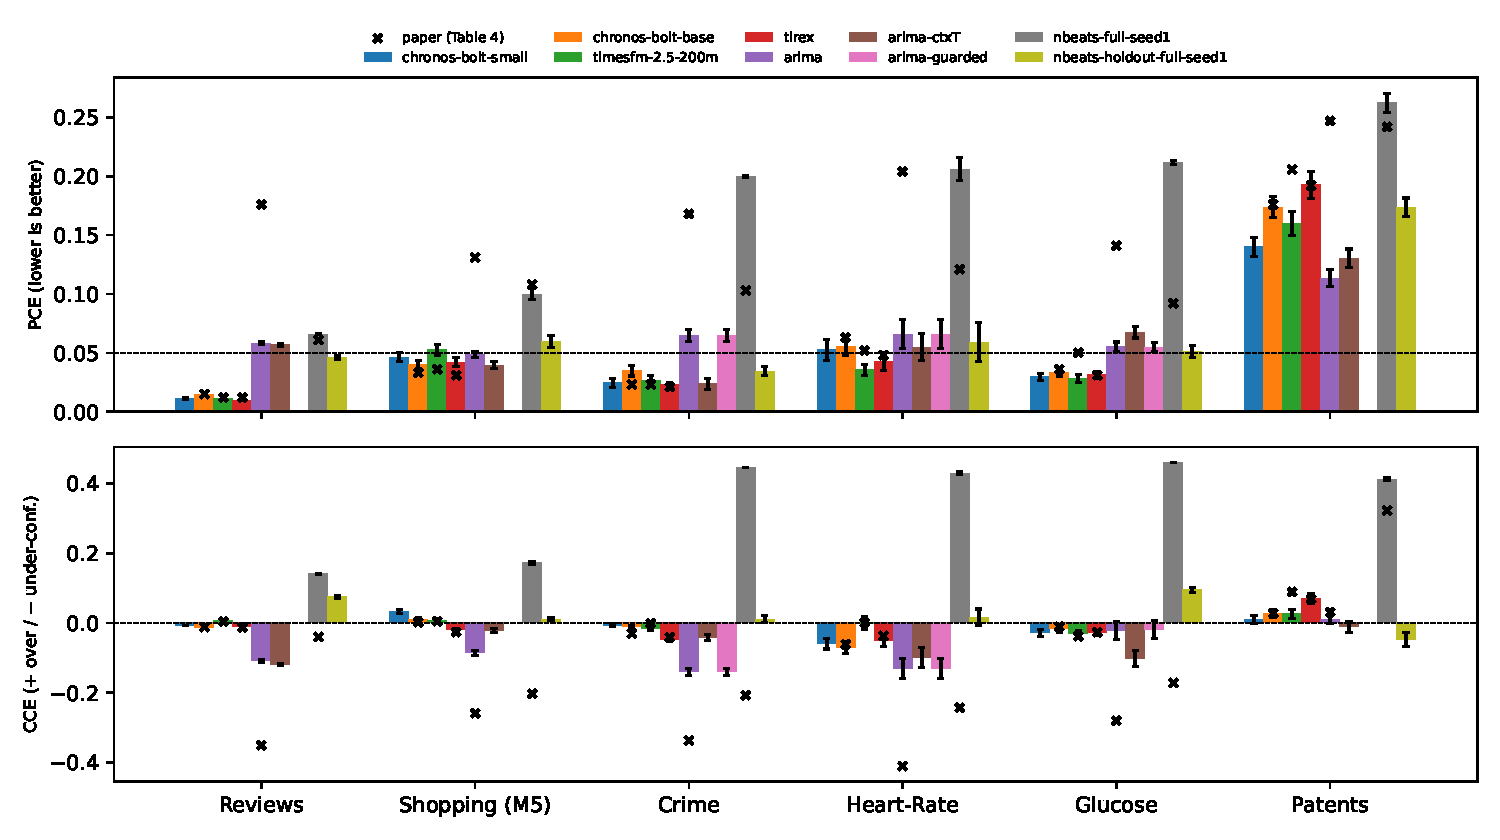
\includegraphics[width=\linewidth]{figures/pce_cce.pdf}
\caption{PCE (top) and signed CCE (bottom) for all six datasets. Bars show this replication (mean $\pm$ SEM across
series). Black crosses show the paper's Table~4 value for the corresponding model: on the Chronos-Bolt-base, TiRex,
ARIMA (64) and N-BEATS (in-sample) bars, and on the TimesFM-2.5 bar for the paper's TimesFM-2.0. The dashed line
marks PCE $=0.05$. Generated by \texttt{src/make\_figures.py}.}
\label{fig:pce}
\end{figure}

\paragraph{C1b (level).} On the five datasets where the paper makes the claim, every TSFM has PCE at or below 0.06:
\begin{itemize}
\item Reviews: \minTSFMpceRev--\maxTSFMpceRev{} (paper's TSFMs: 0.012--0.015);
\item M5: \minTSFMpceMfive--\maxTSFMpceMfive{} (0.031--0.052);
\item Crime: \minTSFMpceCrime--\maxTSFMpceCrime{} (0.014--0.035);
\item Heart-Rate: \minTSFMpceHR--\maxTSFMpceHR{} (0.048--0.077);
\item Glucose: \minTSFMpceGlucose--\maxTSFMpceGlucose{} (0.031--0.050).
\end{itemize}
On Patents, which the paper exempts, our TSFMs reach \minTSFMpcePat--\maxTSFMpcePat, inside the paper's range of
0.154--0.259 or below it. The paper's ranges above are over all five TSFMs of its Table~4.

\paragraph{C1a (ranking).} Against the primary in-sample N-BEATS (full grid), every TSFM has lower PCE on all
six datasets, for every seed (\cOneAholdsFull/\cOneArunsFull{} runs; Table~\ref{tab:seeds}). Against the primary
ARIMA (64) it holds on four of six datasets:
\begin{itemize}
\item it holds on Reviews (ARIMA PCE \pceArimaRev), Crime (\pceArimaCrime), Heart-Rate (\pceArimaHR) and Glucose
(\pceArimaGlucose);
\item it fails on M5, where ARIMA (64) reaches \pceArimaMfive{} and TimesFM-2.5 (\pceTfmMfive) is above it. The
paper's own checkpoints, Chronos-Bolt-base (\pceCbMfive) and TiRex (\pceTrxMfive), are below it;
\item it fails on Patents for every TSFM: ARIMA (64) reaches \pceArimaPat, below the best TSFM
(\minTSFMpcePat).
\end{itemize}
Table~\ref{tab:verdict} lists each comparison, together with the number of series-level wins (TSFM $\times$
series pairs). Where C1a holds, the margin is much smaller than in the paper:
\begin{itemize}
\item The paper's ARIMA PCE is 0.176 (Reviews), 0.131 (M5), 0.168 (Crime), 0.204 (Heart-Rate), 0.141 (Glucose)
and 0.247 (Patents) (Table~4). Our ARIMA (64) is at \pceArimaRev, \pceArimaMfive, \pceArimaCrime,
\pceArimaHR, \pceArimaGlucose{} and \pceArimaPat.
\item The ranking is not robust to the ARIMA refit window. ARIMA ($T$) reaches PCE \pceArimaTCrime{} on Crime,
\pceArimaTHR{} on Heart-Rate and \pceArimaTMfive{} on M5, which is below or level with the worst TSFM
(\maxTSFMpceCrime, \maxTSFMpceHR{} and \maxTSFMpceMfive). On Reviews (\pceArimaTRev) and Glucose
(\pceArimaTGlucose) it stays above every TSFM.
\item N-BEATS with hold-out selection is far better calibrated than in-sample N-BEATS. With the full grid its
mean over seeds is \pceNbeatsFHRevMean{} (Reviews), \pceNbeatsFHMfiveMean{} (M5), \pceNbeatsFHCrimeMean{}
(Crime), \pceNbeatsFHHRMean{} (Heart-Rate), \pceNbeatsFHGlucoseMean{} (Glucose) and \pceNbeatsFHPatMean{}
(Patents). It beats the worst TSFM in \the\numexpr\cOneArunsFullH-\cOneAholdsFullH\relax{} of
\cOneArunsFullH{} runs: all three Crime seeds, one M5 seed and two Patents seeds.
\end{itemize}


\paragraph{Seed variability and selected configurations.}\label{sec:seeds}
Table~\ref{tab:seeds} gives N-BEATS PCE, CCE and MASE as mean $\pm$ SD across seeds 0--2, and the number of seeds
for which C1a holds against that run.

\emph{In-sample selection} is stable. With the full grid, it picks 1000 steps, learning rate $10^{-3}$, blocks
$(3,3,3)$, quantile loss and no early stopping for every one of the six datasets and every seed; only the inert validation-check setting
varies (\texttt{results/runlogs/*full-seed*.json}). That configuration nearly memorises the training windows
(selection WQL \selWQLmin--\selWQLmax{} on the reduced grid), and its PCE SD is at most 0.002.

\emph{Hold-out selection} is seed-sensitive. Its choice changes between seeds: on Crime it picks a Normal-loss
model for all three seeds, and on Glucose seed~0 picks a Normal-loss model with PCE 0.174, hence the large SD.
On Patents the hold-out SD is \pceNbeatsFHPatSD.

C1a holds against full-grid in-sample N-BEATS in \cOneAholdsFull/\cOneArunsFull{} runs, and against full-grid
hold-out N-BEATS in \cOneAholdsFullH/\cOneArunsFullH{} (six datasets $\times$ three seeds). The failures are all
three Crime seeds, M5 seed~2 and Patents seeds 1 and~2. On the reduced grid (Crime, Heart-Rate and Glucose only)
the counts are \cOneAholdsRed/\cOneArunsRed{} (in-sample) and \cOneAholdsRedH/\cOneArunsRedH{} (hold-out).

The TSFMs need no seeds. A repeat of every TSFM on Heart-Rate (\texttt{results/determinism.csv}) gives bitwise
identical quantiles for Chronos-Bolt (small, base) and TimesFM-2.5. TiRex on the CPU torch backend differs only
at floating-point level (median absolute difference 0.002~bpm), and its PCE changes by $1.5\times10^{-5}$.

\begin{table}[h!]\centering\scriptsize\setlength\tabcolsep{3pt}
\begin{tabular}{llcccccc}
\toprule
Dataset & N-BEATS grid, selection & seeds & PCE & CCE & MASE & worst TSFM PCE & C1a holds \\
\midrule
Reviews & full (64), in-sample & 0,1,2 & 0.066$\pm$0.003 & 0.141$\pm$0.006 & 1.035$\pm$0.006 & 0.014 & 3/3 \\
Reviews & full (64), hold-out & 0,1,2 & 0.054$\pm$0.007 & 0.102$\pm$0.023 & 1.168$\pm$0.004 & 0.014 & 3/3 \\
M5 & full (64), in-sample & 0,1,2 & 0.098$\pm$0.002 & 0.169$\pm$0.004 & 0.777$\pm$0.001 & 0.053 & 3/3 \\
M5 & full (64), hold-out & 0,1,2 & 0.056$\pm$0.008 & 0.016$\pm$0.008 & 0.747$\pm$0.019 & 0.053 & 2/3 \\
Crime & reduced (8), in-sample & 0,1,2 & 0.198$\pm$0.002 & 0.441$\pm$0.002 & 0.976$\pm$0.007 & 0.035 & 3/3 \\
Crime & reduced (8), hold-out & 0,1,2 & 0.037$\pm$0.018 & 0.065$\pm$0.050 & 0.828$\pm$0.027 & 0.035 & 1/3 \\
Crime & full (64), in-sample & 0,1,2 & 0.199$\pm$0.001 & 0.444$\pm$0.001 & 0.975$\pm$0.001 & 0.035 & 3/3 \\
Crime & full (64), hold-out & 0,1,2 & 0.026$\pm$0.009 & 0.006$\pm$0.011 & 0.822$\pm$0.008 & 0.035 & 0/3 \\
Heart-Rate & reduced (8), in-sample & 0,1,2 & 0.209$\pm$0.002 & 0.432$\pm$0.001 & 1.654$\pm$0.015 & 0.055 & 3/3 \\
Heart-Rate & reduced (8), hold-out & 0,1,2 & 0.060$\pm$0.002 & 0.018$\pm$0.005 & 1.554$\pm$0.017 & 0.055 & 3/3 \\
Heart-Rate & full (64), in-sample & 0,1,2 & 0.208$\pm$0.002 & 0.432$\pm$0.002 & 1.655$\pm$0.017 & 0.055 & 3/3 \\
Heart-Rate & full (64), hold-out & 0,1,2 & 0.061$\pm$0.002 & 0.018$\pm$0.005 & 1.554$\pm$0.018 & 0.055 & 3/3 \\
Glucose & reduced (8), in-sample & 0,1,2 & 0.212$\pm$0.000 & 0.461$\pm$0.000 & 8.601$\pm$0.057 & 0.033 & 3/3 \\
Glucose & reduced (8), hold-out & 0,1,2 & 0.052$\pm$0.001 & 0.098$\pm$0.001 & 7.839$\pm$0.028 & 0.033 & 3/3 \\
Glucose & full (64), in-sample & 0,1,2 & 0.212$\pm$0.000 & 0.461$\pm$0.001 & 8.651$\pm$0.039 & 0.033 & 3/3 \\
Glucose & full (64), hold-out & 0,1,2 & 0.092$\pm$0.071 & 0.123$\pm$0.046 & 9.129$\pm$2.281 & 0.033 & 3/3 \\
Patents & full (64), in-sample & 0,1,2 & 0.262$\pm$0.009 & 0.417$\pm$0.005 & 15.517$\pm$0.590 & 0.193 & 3/3 \\
Patents & full (64), hold-out & 0,1,2 & 0.190$\pm$0.035 & 0.029$\pm$0.067 & 15.761$\pm$2.737 & 0.193 & 1/3 \\
\bottomrule
\end{tabular}

\caption{N-BEATS across seeds (mean $\pm$ SD over seeds 0--2; \texttt{results/seed\_summary.csv},
\texttt{results/seed\_verdict.csv}). Full (64): the paper's Table~3 grid, run on an Apple M2 Max (MPS). Reduced (8): the
sensitivity grid, run on the CPU box for the first three datasets only. Tables~\ref{tab:mainnew} and~\ref{tab:main} show seed~1. ``C1a holds'' counts
the seeds for which every TSFM has lower PCE than that N-BEATS run.}
\label{tab:seeds}
\end{table}

\paragraph{Sensitivity: ARIMA refit context.}\label{sec:arimactx}
The paper gives two descriptions of the ARIMA context: ``max lag (context) \ldots{} 64'' (App.~A.2) and a refit
``on all earlier data'' (App.~A.4). We therefore repeat ARIMA on Crime, Heart-Rate and Glucose with refit context $W\in\{32,64,128,256,T\}$, where
$T$ is the TSFM context (512 or 128). This grid is our assumption and is not in the paper. The AutoARIMA order is
still selected once on the training split, and only the refit window changes
(\texttt{scripts/run\_arima\_ctx\_sweep.sh}, \texttt{results/arima\_ctx\_sweep.csv}). Table~\ref{tab:arimactx}
and Figure~\ref{fig:arimactx} give the results.
\begin{itemize}
\item \emph{Crime.} PCE falls steadily as $W$ grows, from \ctxPceMaxCrime{} to \ctxPceMinCrime. C1a against ARIMA
fails from $W=256$: one TSFM is beaten at 256 and three of four at $T=512$.
\item \emph{Heart-Rate.} PCE also falls as $W$ grows. C1a fails at $W=T=128$, where ARIMA (0.0547) is just below
the worst TSFM (0.0553, well within one SEM of 0.012).
\item \emph{Glucose.} PCE rises slightly with $W$ (\ctxPceMinGlucose--\ctxPceMaxGlucose), and C1a holds for
every $W$.
\end{itemize}
On Reviews, M5 and Patents we ran only $W\in\{64,T\}$ (Table~\ref{tab:mainnew}).
C1a against ARIMA therefore rests on the short refit context of App.~A.2. Under the App.~A.4 reading
(approximated by $W{=}T$) it fails on four of six datasets: Crime, Heart-Rate, M5 and Patents. The shortest context moves Crime and Heart-Rate ARIMA towards the paper's poorly calibrated,
under-confident ARIMA, but no $W$ reaches the paper's PCE of 0.14--0.20 (Table~4), and on the other three datasets neither
$W{=}64$ nor $W{=}T$ comes near the paper's 0.131--0.247. The context length alone
therefore does not explain the gap.

\begin{table}[h!]\centering\scriptsize
\begin{tabular}{llrrrrl}
\toprule
Dataset & $W$ & PCE & CCE & MASE & TSFMs beaten & C1a \\
\midrule
Crime & 32 & 0.112 & -0.249 & 1.139 & 0/4 & holds \\
 & 64 (primary) & 0.065 & -0.140 & 1.029 & 0/4 & holds \\
 & 128 & 0.037 & -0.078 & 0.976 & 0/4 & holds \\
 & 256 & 0.030 & -0.057 & 0.956 & 1/4 & fails \\
 & 512 ($=T$) & 0.024 & -0.041 & 0.942 & 3/4 & fails \\
 & \multicolumn{6}{l}{\scriptsize TSFM PCE range 0.023--0.035; paper ARIMA 0.168} \\
\midrule
Glucose & 32 & 0.055 & +0.033 & $>$100$^\ddagger$ & 0/4 & holds \\
 & 64 (primary) & 0.055 & -0.022 & $>$100$^\ddagger$ & 0/4 & holds \\
 & 128 & 0.062 & -0.071 & 8.929 & 0/4 & holds \\
 & 256 & 0.066 & -0.108 & 7.990 & 0/4 & holds \\
 & 512 ($=T$) & 0.067 & -0.102 & 8.476 & 0/4 & holds \\
 & \multicolumn{6}{l}{\scriptsize TSFM PCE range 0.028--0.033; paper ARIMA 0.141} \\
\midrule
Heart-Rate & 32 & 0.086 & -0.176 & 2.203 & 0/4 & holds \\
 & 64 (primary) & 0.066 & -0.131 & 1.842 & 0/4 & holds \\
 & 128 ($=T$) & 0.055 & -0.100 & 1.591 & 1/4 & fails \\
 & \multicolumn{6}{l}{\scriptsize TSFM PCE range 0.036--0.055; paper ARIMA 0.204} \\
\bottomrule
\end{tabular}

\caption{ARIMA refit-context sweep (\texttt{results/arima\_ctx\_sweep.csv}). ``TSFMs beaten'' counts TSFMs with
PCE $\geq$ ARIMA($W$). C1a holds if none is beaten. $^\ddagger$A few explosive refits inflate the mean MASE on
Glucose. At $W=64$ the guarded variant (Methods) brings MASE to 8.472 and changes PCE only from 0.0551 to 0.0549.}
\label{tab:arimactx}
\end{table}
\begin{figure}[h!]\centering
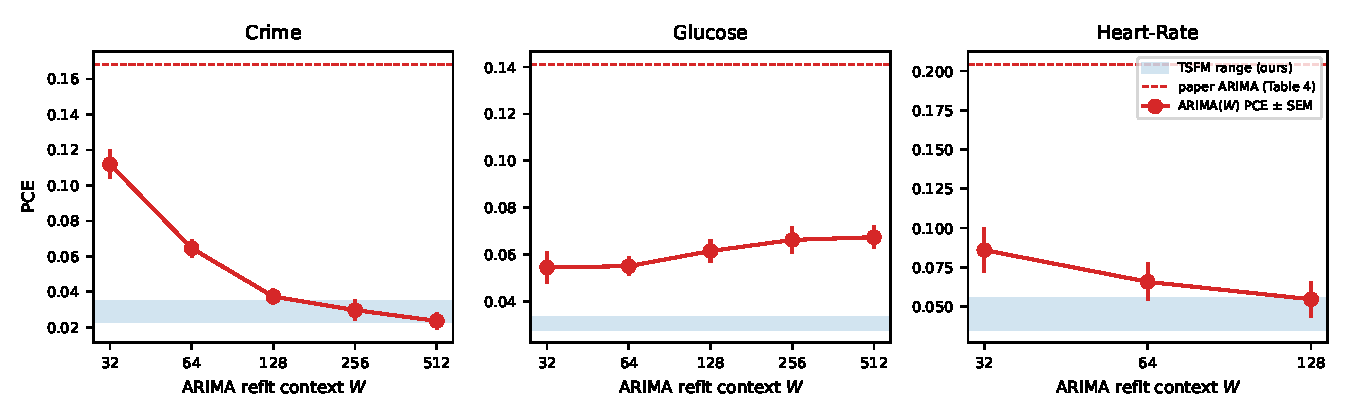
\includegraphics[width=\linewidth]{figures/arima_ctx.pdf}
\caption{ARIMA PCE ($\pm$ SEM across series) against the refit context $W$. The shaded band is the range of our
four TSFMs; the dashed line is the paper's ARIMA (Table~4).}
\label{fig:arimactx}
\end{figure}

\paragraph{Supporting observations.}
\begin{itemize}
\item \textbf{Direction of the baselines' errors.} Like the paper, we find ARIMA (64) under-confident (negative
CCE) on five datasets, but less so: for example, Crime \cceArimaCrime{} against the paper's $-0.337$, and Reviews
\cceArimaRev{} against $-0.351$. On Patents both the paper's ARIMA (0.031) and ours (\cceArimaPat) are slightly
positive.
\item \textbf{N-BEATS.} Unlike the paper, our in-sample N-BEATS is \emph{overconfident} on Reviews, M5, Crime,
Heart-Rate and Glucose, and the full grid does not change this. Full-grid in-sample CCE averages
\cceNbeatsFRevMean{} (Reviews), \cceNbeatsFMfiveMean{} (M5), \cceNbeatsFCrimeMean{} (Crime),
\cceNbeatsFHRMean{} (Heart-Rate) and \cceNbeatsFGlucoseMean{} (Glucose), against the paper's $-0.040$, $-0.203$,
$-0.207$, $-0.243$ and $-0.172$. On Patents both are overconfident (ours \cceNbeatsFPatMean, paper 0.322). Among all
\the\numexpr\cOneArunsRed+\cOneArunsRedH+\cOneArunsFull+\cOneArunsFullH\relax{} full- and reduced-grid runs,
CCE is negative only in \cceNegFullH{} full-grid hold-out runs (Crime seed~2 and Patents seed~1).
\item \textbf{TSFMs.} The TSFMs show no consistent CCE sign, in line with the paper.
\item \textbf{MASE.} Our TSFM MASE differs from Table~4 in level: higher on Reviews, Crime, Heart-Rate and Glucose,
about level on M5 and lower on Patents. On the first three datasets we traced this to a difference in definition
(Section~\ref{sec:diag}); we did not repeat that diagnosis on the other three.
\end{itemize}

\paragraph{Validity of the forecasts run on the M2 Max.}\label{sec:validity}
Reviews, M5 and Patents were forecast on another machine, so before using them we checked them against the
code and data in this repository. The checks are in \texttt{scripts/verify\_returned\_forecasts.py} and
\texttt{scripts/verify\_returned\_stage2.py}, and their outputs in \texttt{results/stage1\_validity/}.
\begin{itemize}
\item \emph{Code and data.} The source, scripts, environment pins, data checksums and model revisions in both
returned packages are byte-identical to the repository. The data checksums matched on both machines.
\item \emph{M5 and Patents (forecasts returned).} For all 24 runs the windows (target, series, origin) equal a
rebuild on our machine (\winEqPat{} Patents, \winEqMfive{} M5), quantiles are finite and sorted, and $T$, $L$
match Table~2. Re-evaluating the returned forecasts here reproduces the returned metrics exactly (max relative
difference \reevalMaxDiff). Every N-BEATS run scored all 64 configurations and kept the argmin-WQL configuration.
\item \emph{TSFMs.} We re-forecast windows on our CPU at the pinned revisions (Table~\ref{tab:validity}).
Chronos-Bolt and TimesFM-2.5 agree to $1.5\times10^{-5}$ relative error with identical coverage indicators. TiRex,
which ran on MPS, differs at float level (relative error up to 0.05 on 1{,}024 windows), but at least 99.9\% of coverage
indicators agree and PCE on those windows agrees to within 0.0001.
\item \emph{ARIMA.} AutoARIMA re-selects the same orders on Patents (\arimaOrdersEqPat) but not on two M5 series
(\arimaOrdersEqMfive), and short spot re-forecasts differ. We attribute this to the platforms' floating-point arithmetic:
every affected window is a high-order fit on a short context, where small numerical differences move the
optimiser to a different optimum. We therefore re-ran all four
M5/Patents ARIMA runs in full on our x86 machine. PCE changes by at most \pceBoxDiffArimaMfive{} (M5 ARIMA (64))
and no verdict changes (\texttt{results/stage1\_validity/arima\_crossplatform.csv}, \texttt{*-box} rows of
\texttt{results/verdict.csv}). The tables use the M2 Max runs.
\item \emph{Reviews (no forecasts returned).} The Reviews forecast files were not in the returned package, so
Reviews cannot be re-evaluated or re-forecast here. We checked what the files allow: every run covers all \nwinRev{} windows,
the TSFM model ids match, all six N-BEATS runs scored 64 configurations and kept the argmin, and the returned
summary equals the mean of the returned per-series metrics. The Reviews numbers are therefore the least
independently verified in this report.
\end{itemize}
None of the returned forecasts failed a check that would require a re-run.

\begin{table}[h!]\centering\scriptsize\setlength\tabcolsep{3pt}
\begin{tabular}{lllccc}
\toprule
Dataset & Model & check & max rel.\ err. / result & coverage agr. & PCE Mac / box \\
\midrule
Patents & Chronos-Bolt-S & re-forecast 32 windows (CPU) & 7.4e-06 & 1.0000 & 0.0405 / 0.0405 \\
Patents & Chronos-Bolt-B & re-forecast 32 windows (CPU) & 9.9e-06 & 1.0000 & 0.0197 / 0.0197 \\
Patents & TimesFM-2.5$^\dagger$ & re-forecast 32 windows (CPU) & 1.5e-05 & 1.0000 & 0.0174 / 0.0174 \\
Patents & TiRex & re-forecast 32 windows (CPU) & 6.1e-03 & 0.9989 & 0.0152 / 0.0151 \\
Patents & TiRex & re-forecast 1024 windows (CPU) & 3.4e-02 & 0.9993 & 0.0745 / 0.0745 \\
Patents & ARIMA (64) & full re-run on x86 box & 2.1e-02 (32 win.)$^\S$ & -- & 0.1135 / 0.1135 \\
Patents & ARIMA ($T$)$^\ast$ & full re-run on x86 box & 6.5e-03 (32 win.)$^\S$ & -- & 0.1302 / 0.1302 \\
Patents & N-BEATS (6 runs) & grid 64/64, selection = argmin WQL & 6/6, 6/6 & -- & -- \\
\midrule
M5 & Chronos-Bolt-S & re-forecast 32 windows (CPU) & 2.1e-06 & 1.0000 & 0.0214 / 0.0214 \\
M5 & Chronos-Bolt-B & re-forecast 32 windows (CPU) & 2.1e-06 & 1.0000 & 0.0135 / 0.0135 \\
M5 & TimesFM-2.5$^\dagger$ & re-forecast 32 windows (CPU) & 3.8e-06 & 1.0000 & 0.0105 / 0.0105 \\
M5 & TiRex & re-forecast 32 windows (CPU) & 1.9e-02 & 0.9989 & 0.0086 / 0.0087 \\
M5 & TiRex & re-forecast 1024 windows (CPU) & 4.9e-02 & 0.9990 & 0.0153 / 0.0153 \\
M5 & ARIMA (64) & full re-run on x86 box & 5.6e-01 (32 win.)$^\S$ & -- & 0.0486 / 0.0480 \\
M5 & ARIMA ($T$)$^\ast$ & full re-run on x86 box & 1.8e-02 (32 win.)$^\S$ & -- & 0.0396 / 0.0394 \\
M5 & N-BEATS (6 runs) & grid 64/64, selection = argmin WQL & 6/6, 6/6 & -- & -- \\
\bottomrule
\end{tabular}

\caption{Checks on the forecasts returned from the M2 Max. Source: \texttt{results/stage1\_validity/}. TSFM rows
re-forecast the first windows on our CPU at the pinned revision and compare quantiles (max relative error), the
coverage indicators $\mathbf 1\{y\le\hat y^q\}$ and the pooled PCE over the same windows. ARIMA rows give the
re-forecast error on 32 windows ($^\S$platform-dependent optimiser, see text) and the dataset PCE of the full
re-run on x86. N-BEATS: grid complete, selected configuration is the argmin of the selection WQL.}
\label{tab:validity}
\end{table}

\section{Diagnosis against the authors' code}
\label{sec:diag}

Only after the results above existed did we inspect the authors' repository\supercite{authorsrepo}
(commit \texttt{b60bfd9}). We copied no code into the pipeline. The full notes are in \texttt{DIAGNOSIS.md}.
Table~\ref{tab:diag} recomputes some of our forecasts in two ways:
\begin{itemize}
\item with the authors' aggregation, which we re-implemented from their metric definitions;
\item on the authors' released Crime and Heart-Rate data, run through our pipeline.
\end{itemize}
This diagnosis covers the first three datasets only. Reviews and Patents already use the authors' data, and our M5
equals theirs.

\begin{table}[h!]\centering\scriptsize\setlength\tabcolsep{3pt}
\begin{tabular}{lllcccccc}
\toprule
 & & & \multicolumn{2}{c}{PCE} & \multicolumn{2}{c}{MASE} & \multicolumn{2}{c}{Paper T4} \\
\cmidrule(lr){4-5}\cmidrule(lr){6-7}\cmidrule(lr){8-9}
Dataset & data & Model & ours & authors' agg. & ours & authors' agg. & PCE & MASE \\
\midrule
Crime & ours & Chronos-Bolt-S & 0.024 & 0.024 & 0.80 & 0.74 & -- & -- \\
Crime & ours & TimesFM-2.5$^\dagger$ & 0.027 & 0.026 & 0.78 & 0.72 & 0.023 & 0.76 \\
Crime & ours & ARIMA (64) & 0.065 & 0.065 & 1.03 & 0.97 & 0.168 & 0.83 \\
Crime & ours & ARIMA ($T$)$^\ast$ & 0.024 & 0.023 & 0.94 & 0.89 & 0.168 & 0.83 \\
Crime & authors' & Chronos-Bolt-S & 0.014 & 0.013 & 0.83 & 0.74 & -- & -- \\
Crime & authors' & TimesFM-2.5$^\dagger$ & 0.019 & 0.018 & 0.81 & 0.73 & 0.023 & 0.76 \\
Crime & authors' & ARIMA (64) & 0.065 & 0.065 & 0.99 & 0.91 & 0.168 & 0.83 \\
Crime & authors' & ARIMA ($T$)$^\ast$ & 0.028 & 0.027 & 0.91 & 0.83 & 0.168 & 0.83 \\
Heart-Rate & ours & Chronos-Bolt-S & 0.053 & 0.048 & 1.55 & 1.26 & -- & -- \\
Heart-Rate & ours & TimesFM-2.5$^\dagger$ & 0.036 & 0.015 & 1.47 & 1.18 & 0.052 & 1.10 \\
Heart-Rate & ours & ARIMA (64) & 0.066 & 0.064 & 1.84 & 1.54 & 0.204 & 1.12 \\
Heart-Rate & ours & ARIMA ($T$)$^\ast$ & 0.055 & 0.050 & 1.59 & 1.30 & 0.204 & 1.12 \\
Heart-Rate & authors' & Chronos-Bolt-S & 0.060 & 0.044 & 1.29 & 1.12 & -- & -- \\
Heart-Rate & authors' & TimesFM-2.5$^\dagger$ & 0.053 & 0.018 & 1.26 & 1.09 & 0.052 & 1.10 \\
Heart-Rate & authors' & ARIMA (64) & 0.066 & 0.059 & 1.57 & 1.37 & 0.204 & 1.12 \\
Heart-Rate & authors' & ARIMA ($T$)$^\ast$ & 0.063 & 0.055 & 1.35 & 1.18 & 0.204 & 1.12 \\
\bottomrule
\end{tabular}

\caption{Diagnosis only. ``authors' agg.'' = PCE pooled over the whole dataset; MASE with a global in-sample naive
denominator, clipped at 50 (authors' \texttt{src/metrics.py}). Sources: \texttt{results/diagnosis\_authors\_style\_metrics.csv} and
\texttt{results/summary.csv} (rows \texttt{*\_authorsdata}).}
\label{tab:diag}
\end{table}

\begin{enumerate}
\item \textbf{PCE aggregation.} The authors pool the indicators over all series, windows and horizons, then
average over $q$. This is close to our primary reading. For example, on Crime the two readings agree to about
0.001 for every model. The literal per-window reading is not what the authors compute.
\item \textbf{MASE.} The authors scale by a single in-sample one-step naive MAE pooled over all series, and clip
at 50. With this definition our TSFM MASE values fall into the paper's ranges (Table~\ref{tab:diag}). The MASE gap
is therefore definitional.
\item \textbf{Data.} We compared our data with the authors' releases:
\begin{itemize}
\item Heart-Rate: the authors use the same six subjects as we do, but on a 1-second grid (598 steps) instead of
beat index.
\item Glucose: the authors align subjects on relative time, which confirms our assumption.
\item Crime: the counts differ (correlation 0.72--0.85), which suggests the authors used complaint occurrence date
where we used report date.
\end{itemize}
On the authors' data, the qualitative picture is unchanged.
\item \textbf{ARIMA and N-BEATS: not resolved.} The repository contains no baseline code, so the large gap
between our ARIMA (PCE $\approx0.06$) and the paper's (0.14--0.20) cannot be explained from the code. The same
holds for the opposite CCE sign of our N-BEATS. The gap persists on the authors' data and under their aggregation.
\end{enumerate}

\section{Verdict}

\begin{table}[h!]\centering\scriptsize\setlength\tabcolsep{3pt}
\begin{tabular}{llcccc}
\toprule
Dataset & Test & max TSFM PCE & baseline PCE & series-pair wins & holds \\
\midrule
Reviews & C1a vs ARIMA (64) & 0.014 & 0.058 & 932/940 & yes \\
Reviews & C1a vs ARIMA ($T$)$^\ast$ & 0.014 & 0.057 & 936/940 & yes \\
Reviews & C1a vs N-BEATS (full, in-sample) & 0.014 & 0.066 & 939/940 & yes \\
Reviews & C1a vs N-BEATS (full, hold-out)$^\ast$ & 0.014 & 0.046 & 880/940 & yes \\
Reviews & C1b (max TSFM PCE $\le$ 0.06) & 0.014 & -- & -- & yes \\
M5 & C1a vs ARIMA (64) & 0.052 & 0.049 & 156/280 & no \\
M5 & C1a vs ARIMA ($T$)$^\ast$ & 0.052 & 0.040 & 125/280 & no \\
M5 & C1a vs N-BEATS (full, in-sample) & 0.052 & 0.100 & 277/280 & yes \\
M5 & C1a vs N-BEATS (full, hold-out)$^\ast$ & 0.052 & 0.060 & 192/280 & yes \\
M5 & C1b (max TSFM PCE $\le$ 0.06) & 0.052 & -- & -- & yes \\
Crime & C1a vs ARIMA (64) & 0.035 & 0.065 & 20/20 & yes \\
Crime & C1a vs ARIMA ($T$)$^\ast$ & 0.035 & 0.024 & 7/20 & no \\
Crime & C1a vs ARIMA (64, guard)$^\ast$ & 0.035 & 0.065 & 20/20 & yes \\
Crime & C1a vs N-BEATS (full, in-sample) & 0.035 & 0.200 & 20/20 & yes \\
Crime & C1a vs N-BEATS (full, hold-out)$^\ast$ & 0.035 & 0.034 & 17/20 & no \\
Crime & C1a vs N-BEATS (reduced, in-s.)$^\ast$ & 0.035 & 0.199 & 20/20 & yes \\
Crime & C1a vs N-BEATS (reduced, hold-out)$^\ast$ & 0.035 & 0.058 & 20/20 & yes \\
Crime & C1b (max TSFM PCE $\le$ 0.06) & 0.035 & -- & -- & yes \\
Heart-Rate & C1a vs ARIMA (64) & 0.055 & 0.066 & 20/24 & yes \\
Heart-Rate & C1a vs ARIMA ($T$)$^\ast$ & 0.055 & 0.055 & 17/24 & no \\
Heart-Rate & C1a vs ARIMA (64, guard)$^\ast$ & 0.055 & 0.066 & 20/24 & yes \\
Heart-Rate & C1a vs N-BEATS (full, in-sample) & 0.055 & 0.206 & 24/24 & yes \\
Heart-Rate & C1a vs N-BEATS (full, hold-out)$^\ast$ & 0.055 & 0.059 & 15/24 & yes \\
Heart-Rate & C1a vs N-BEATS (reduced, in-s.)$^\ast$ & 0.055 & 0.207 & 24/24 & yes \\
Heart-Rate & C1a vs N-BEATS (reduced, hold-out)$^\ast$ & 0.055 & 0.059 & 15/24 & yes \\
Heart-Rate & C1b (max TSFM PCE $\le$ 0.06) & 0.055 & -- & -- & yes \\
Glucose & C1a vs ARIMA (64) & 0.033 & 0.055 & 56/64 & yes \\
Glucose & C1a vs ARIMA ($T$)$^\ast$ & 0.033 & 0.067 & 64/64 & yes \\
Glucose & C1a vs ARIMA (64, guard)$^\ast$ & 0.033 & 0.055 & 56/64 & yes \\
Glucose & C1a vs N-BEATS (full, in-sample) & 0.033 & 0.212 & 64/64 & yes \\
Glucose & C1a vs N-BEATS (full, hold-out)$^\ast$ & 0.033 & 0.051 & 57/64 & yes \\
Glucose & C1a vs N-BEATS (reduced, in-s.)$^\ast$ & 0.033 & 0.212 & 64/64 & yes \\
Glucose & C1a vs N-BEATS (reduced, hold-out)$^\ast$ & 0.033 & 0.054 & 57/64 & yes \\
Glucose & C1b (max TSFM PCE $\le$ 0.06) & 0.033 & -- & -- & yes \\
Patents & C1a vs ARIMA (64) & 0.193 & 0.114 & 102/332 & no \\
Patents & C1a vs ARIMA ($T$)$^\ast$ & 0.193 & 0.130 & 138/332 & no \\
Patents & C1a vs N-BEATS (full, in-sample) & 0.193 & 0.262 & 267/332 & yes \\
Patents & C1a vs N-BEATS (full, hold-out)$^\ast$ & 0.193 & 0.174 & 197/332 & no \\
Patents & C1b (max TSFM PCE $\le$ 0.06) & 0.193 & -- & -- & no (not claimed) \\
\bottomrule
\end{tabular}

\caption{Per-dataset checks of C1a and C1b (\texttt{results/verdict.csv}; N-BEATS rows are seed~1). ``Series-pair
wins'' counts the (TSFM, series) pairs in which the TSFM has lower per-series PCE than the baseline. ``Not
claimed'': the paper exempts Patents from C1b (\S4.1).}
\label{tab:verdict}
\end{table}

\begin{itemize}
\item \textbf{C1b (TSFM PCE close to or below 5\%): reproduced} on all five datasets where the paper claims it
(Reviews, M5, Crime, Heart-Rate, Glucose), with four TSFMs including a substitute TimesFM. On Patents, which the
paper exempts, our TSFM PCE (\minTSFMpcePat--\maxTSFMpcePat) is as high as the paper's.
\item \textbf{C1a (TSFMs better calibrated than the baselines): partially reproduced.}
\begin{itemize}
\item Against full-grid N-BEATS with in-sample selection, every TSFM has lower PCE on all six datasets and for
every seed.
\item Against ARIMA (64), every TSFM has lower PCE on Reviews, Crime, Heart-Rate and Glucose. On M5 the
substitute TimesFM-2.5 is above ARIMA (64), and on Patents every TSFM is.
\item Where it holds, the margin is a fraction of the paper's: our ARIMA is far better calibrated than the
paper's on every dataset.
\item An ARIMA refit on the same context as the TSFMs matches or beats some TSFMs on Crime, Heart-Rate, M5 and
Patents.
\item With hold-out selection, N-BEATS beats the worst TSFM on Crime (all seeds), M5 (one seed) and Patents
(two seeds).
\item The paper's very poorly calibrated baselines could not be reproduced, and the released code does not
include the baselines.
\end{itemize}
\end{itemize}
Overall verdict on the main calibration claim: \textbf{partially reproduced}.

\section{Deviations, limitations and incomplete items}
\label{sec:incomplete}
\begin{itemize}
\item \textbf{Model substitution.} TimesFM-2.5-200M replaces TimesFM-2.0-500M. Moirai~2.0 and YingLong were not run.
\item \textbf{N-BEATS grid.} The full Table~3 grid was run, but the paper does not describe how early stopping
gets its validation data, and our choice is an assumption. Full-grid runs used MPS, other runs the CPU; GPU
training is not bit-for-bit reproducible.
\item \textbf{Datasets.} All six real datasets are tested. The stride is assumed (A-01), and our forecast counts
differ from Table~1 on M5 and Patents (Methods). Reviews has 235 series instead of 239. Data construction for
Crime, Heart-Rate and Glucose differs from the authors' releases as described in Section~\ref{sec:diag}.
\item \textbf{Hardware.} Crime, Heart-Rate and Glucose ran on a CPU machine, except the full N-BEATS grid.
Reviews, M5 and Patents ran entirely on an Apple M2 Max: Chronos-Bolt, TiRex and N-BEATS on MPS, TimesFM-2.5 on the
CPU (MPS has no float64), ARIMA on the CPU. TiRex never used its CUDA kernels.
\item \textbf{Metric levels.} SIW and WQL use definitions that differ in absolute level from the authors' code.
Neither is part of the tested claim.
\item \textbf{Uncertainty.} The TSFM and ARIMA values come from one deterministic run each, so their uncertainty is
the SEM across series. N-BEATS also has an SD across 3 seeds (Table~\ref{tab:seeds}).
\end{itemize}

\paragraph{Limitations and anticipated questions.}\label{sec:limits}
\begin{itemize}
\item \emph{Reviews is checked less than the other datasets.} Its forecasts were not returned, so its metrics come
from the same \texttt{evaluate.py} run on the M2 Max and are merged as returned
(\texttt{src/evaluate.py -{}-include-returned results/stage2}). Section~\ref{sec:validity} lists what was checked.
\item \emph{Patents.} The paper exempts Patents from the 5\% level, and its own YingLong PCE (0.259) there is above
both baselines (0.242, 0.247). Our Patents result, ARIMA better calibrated than every TSFM, is the clearest
contradiction of C1a in this report, but it rests on a baseline that is far better calibrated than the paper's.
\item \emph{Model versions and sizes.} TimesFM-2.5-200M replaces the paper's TimesFM-2.0-500M (different
architecture, smaller model). Chronos-Bolt is run in its small and base sizes. TiRex is run in its only released
size. Moirai~2.0 and YingLong are not run. C1b holds for the paper's own Chronos-Bolt-base and TiRex checkpoints,
so the substitute does not drive it. C1a, the per-model ranking, is not tested for TimesFM-2.0 itself.
\item \emph{TiRex backend.} TiRex ran on its torch backend (CPU, or MPS for Reviews, M5 and Patents) instead of the
CUDA kernels. On a CPU repeat it differs from itself only at float level (PCE changes by $1.5\times10^{-5}$), and
MPS and CPU agree to within 0.0001 in PCE (Table~\ref{tab:validity}), but we cannot rule out a larger
difference from the CUDA kernels.
\item \emph{Aggregation choices.} Eq.~1 does not say how PCE is aggregated over series, windows and horizons. We
report the mean over series (assumption A1) and check the authors' pooled reading in Section~\ref{sec:diag}. The
two agree to about 0.001 on Crime. MASE levels depend on the scaling denominator. Neither choice changes the
ranking we report.
\item \emph{Crime data.} We count complaints by report date. The authors' release correlates only 0.72--0.85 with
our counts, which suggests they used occurrence date. On their data the qualitative picture is the same
(Table~\ref{tab:diag}).
\item \emph{ARIMA context.} The paper gives two conflicting descriptions: a context of 64 (App.~A.2) and a refit
on all earlier data (App.~A.4). We take 64 as primary and sweep the refit context in
Section~\ref{sec:arimactx}. The sweep shows how far the C1a result against ARIMA depends on this setting.
\item \emph{N-BEATS sign gap.} Our N-BEATS is overconfident, while the paper's is under-confident on five of six
datasets. This holds on both grids, both selection readings and all three seeds, with two hold-out exceptions, and we have no explanation, because the baseline code is
not released.
\item \emph{No author contact.} We deliberately did not contact the authors. Every gap above is therefore resolved,
if at all, only from the paper, the public repository and the public data. An author's answer could settle the
ARIMA context, the N-BEATS early-stopping split and the Crime date field.
\end{itemize}

\section{Reproducibility}\label{sec:repro}
The code, environment pins (\texttt{envs/}), model revisions (\texttt{envs/MODEL\_REVISIONS.md}) and run logs
(\texttt{results/runlogs/}) are in the repository. \texttt{README.md} and \texttt{REPRODUCE.md} give the commands
that regenerate every number and figure in this article from raw public data or the authors' released data.
\begin{itemize}
\item \emph{Software.} One Python virtual environment per model family (Chronos-Bolt, TimesFM, TiRex, StatsForecast,
NeuralForecast), with exact pins in \texttt{envs/requirements-*.txt}: Python~3.11.17 with torch~2.5.1 (CPU wheels)
on the CPU machine, and Python~3.12.11 with torch~2.5.1 on the M2 Max. Hugging Face checkpoints are pinned by
revision hash in \texttt{envs/MODEL\_REVISIONS.md}.
\item \emph{Data.} Raw data are not redistributed in the repository. \texttt{scripts/fetch\_raw\_data.sh} downloads
the Crime, Heart-Rate and Glucose files and checks them against \texttt{data/raw/SHA256SUMS.txt};
\texttt{scripts/prepare\_data.py} downloads Reviews, M5 and Patents from pinned sources and checks the processed
files against \texttt{data/processed/CHECKSUMS.sha256}. The NYPD source is a live dataset, so a later download
can differ from ours; the checksum check reports this.
\item \emph{Outputs.} Forecast arrays (\texttt{results/forecasts/}) are too large for the repository and are not
included. The per-series and per-dataset metrics from which all tables, figures and verdicts are built are
included (\texttt{results/}), and \texttt{scripts/make\_tables.py} regenerates the article tables from them.
\end{itemize}
Hardware:
\begin{itemize}
\item Crime, Heart-Rate and Glucose, except the full N-BEATS grid, ran on a shared 8-core CPU machine with no GPU,
with at most 4 threads per process.
\item The full grid for those three datasets (18 runs) ran on an Apple M2 Max (32\,GB) with PyTorch~2.5.1 on MPS,
Python~3.12 and NeuralForecast~3.1.9 (\texttt{results/runlogs/gpu\_env.txt}). It took 3\,h\,14\,min wall-clock in
one uninterrupted pass, 533--1313\,s per run (\texttt{results/runlogs\_nbeats\_full.txt}). It was started with
\texttt{bash run\_gpu.sh}, with code identical to the repository at commit \texttt{3e54d0c}.
\item Reviews, M5 and Patents ran on the same M2 Max (Python~3.12.11, PyTorch~2.5.1) with
\texttt{bash run\_stage1.sh} (Patents, M5) and \texttt{bash run\_stage2.sh} (Reviews), with code identical to
commit \texttt{3dddf5f} (\texttt{STAGES.md}; logs \texttt{results/runlogs\_stage1.txt},
\texttt{results/runlogs\_stage2.txt}, environments \texttt{results/runlogs/env\_stage\{1,2\}/}). The runner checks
the device per model on 16 windows against the CPU and falls back to the CPU if they disagree or the device fails.
\item The ARIMA cross-platform re-runs for M5 and Patents (\texttt{*-box}) ran on the CPU machine.
\end{itemize}

\section*{AI-assistance disclosure}
The author used Grok 4.7 in preparing this replication.
